\documentclass[12pt]{article}

\usepackage[a4paper, margin=1in]{geometry}
\usepackage{graphicx}
\usepackage{titlesec}
\usepackage{enumitem}
\usepackage{amsmath}
\usepackage{booktabs}
\usepackage{xcolor}
\usepackage{hyperref}
\usepackage{graphicx}

\title{
\Huge \textbf{Human-Centered Artificial Intelligence (HCAI)} \\
\vspace{0.5cm}
\LARGE Heart Disease Prediction System
}

\author{}
\date{}
\usepackage{fancyhdr}

\pagestyle{fancy}
\fancyhf{}

% Header
\lhead{Human-Centered Artificial Intelligence (HCAI)}
\rhead{Heart Disease Prediction System}

% Footer
\lfoot{\thepage}
\rfoot{2026}

% Header/Footer line
\renewcommand{\headrulewidth}{0.5pt}
\renewcommand{\footrulewidth}{0.5pt}
\begin{document}

\maketitle

\section*{Abstract}

This report presents a Human-Centered AI (HCAI) based Heart Disease Prediction System implemented as a Streamlit web application. The project combines machine learning algorithms with an interactive user interface to assist users in identifying possible heart disease risks. The system emphasizes human oversight, transparency, ethical AI principles, and healthcare accessibility. Multiple machine learning algorithms were evaluated and compared, and the Random Forest Classifier was selected as the final deployed model due to its superior performance. The project aligns with Sustainable Development Goals related to health, education, and innovation.

\section*{Introduction}

Heart disease is one of the leading causes of death worldwide. Early risk identification can help individuals seek preventive healthcare and improve medical outcomes. This project demonstrates how machine learning and Human-Centered AI principles can be applied to healthcare support systems.

The application is designed around the principles of Human-Centered AI:
\begin{itemize}
    \item Transparency
    \item User control
    \item Ethical AI usage
    \item Human oversight
    \item Accessibility
\end{itemize}

The system collects patient health metrics, preprocesses the input data, and uses a trained machine learning model to predict the probability of heart disease risk. The prediction is advisory in nature and is intended to support awareness rather than replace professional medical diagnosis.

\section*{Project Overview}

\textbf{Project Name:} Heart Disease Prediction System

\textbf{Implementation:}
Python Streamlit application with machine learning based heart disease prediction.

\section*{Primary Functions}

\begin{itemize}
    \item Collect patient health indicators through a web interface.
    \item Preprocess user inputs for machine learning inference.
    \item Predict heart disease risk using a trained classifier.
    \item Display risk probability and risk category using visual indicators.
    \item Support healthcare awareness through understandable outputs.
\end{itemize}

\section*{Target Users}

\begin{itemize}
    \item Students learning Machine Learning and HCAI concepts.
    \item Healthcare support practitioners.
    \item Users interested in basic heart disease risk awareness.
\end{itemize}

\section*{Technologies Used}

\begin{table}[h]
\centering
\begin{tabular}{ll}
\toprule
\textbf{Technology} & \textbf{Purpose} \\
\midrule
Python & Core programming language \\
Pandas & Data preprocessing and handling \\
Scikit-learn & Machine learning algorithms \\
Streamlit & Frontend web application \\
Matplotlib & Data visualization \\
Seaborn & Correlation heatmaps and plots \\
LabelEncoder & Categorical data encoding \\
\bottomrule
\end{tabular}
\end{table}

\section*{Machine Learning Algorithms Used}

The following machine learning algorithms were implemented and compared:

\begin{enumerate}
    \item Logistic Regression
    \item Decision Tree Classifier
    \item K-Nearest Neighbour (KNN)
    \item Random Forest Classifier
\end{enumerate}

The algorithms were evaluated using:
\begin{itemize}
    \item Accuracy
    \item Precision
    \item Recall
    \item F1-Score
\end{itemize}

The Random Forest Classifier achieved the highest accuracy and was selected as the final model for deployment.

\section*{Human and Computer Automation Levels}

This system follows a collaborative automation model with strong human oversight.

\subsection*{Human Role}

\begin{itemize}
    \item Enters patient health information.
    \item Initiates prediction manually.
    \item Reviews risk probability and prediction results.
    \item Makes the final healthcare decisions.
\end{itemize}

\subsection*{Computer Role}

\begin{itemize}
    \item Processes user inputs.
    \item Executes machine learning inference.
    \item Predicts heart disease risk.
    \item Displays probability and risk level.
\end{itemize}

\subsection*{Automation Level (HCAI Perspective)}

\begin{itemize}
    \item Human-led interaction and decision-making.
    \item Computer-assisted prediction execution.
    \item Advisory output instead of autonomous decision-making.
\end{itemize}

The project therefore operates in a human-in-the-loop framework where AI supports analysis while humans retain control.

\section*{SDG Mapping}

\subsection*{SDG 3: Good Health and Well-being}

\begin{itemize}
    \item Supports early detection of heart disease risks.
    \item Encourages preventive healthcare awareness.
    \item Promotes healthcare accessibility through AI systems.
\end{itemize}

\subsection*{SDG 4: Quality Education}

\begin{itemize}
    \item Demonstrates practical applications of machine learning.
    \item Supports educational learning in AI and HCAI.
    \item Provides an interactive healthcare AI learning platform.
\end{itemize}

\subsection*{SDG 9: Industry, Innovation and Infrastructure}

\begin{itemize}
    \item Showcases digital healthcare innovation using accessible web-based AI.
    \item Encourages reproducible deployment of machine learning models.
    \item Demonstrates lightweight healthcare infrastructure using AI.
\end{itemize}

\subsection*{SDG 10: Reduced Inequalities}

\begin{itemize}
    \item Provides accessible healthcare support tools.
    \item Uses a simple and understandable user interface.
    \item Promotes healthcare technology accessibility for non-technical users.
\end{itemize}

\section*{Implementation Artifacts}

\subsection*{Frontend Application}

The system frontend was developed using Streamlit and includes:

\begin{itemize}
    \item Interactive patient detail forms
    \item Healthcare-focused dashboard interface
    \item Prediction result cards
    \item Risk probability metrics
    \item Demo patient profiles
    \item Color-coded risk indicators
\end{itemize}
\section*{Implementation Artifacts}

\subsection*{Frontend Application Interface}

The frontend application was developed using Streamlit with a healthcare-oriented dashboard design. The interface allows users to enter patient health information such as age, cholesterol level, blood pressure, heart rate, and exercise angina status. The system also includes demo patient profiles for testing different healthcare scenarios.

\begin{figure}[h]
\centering
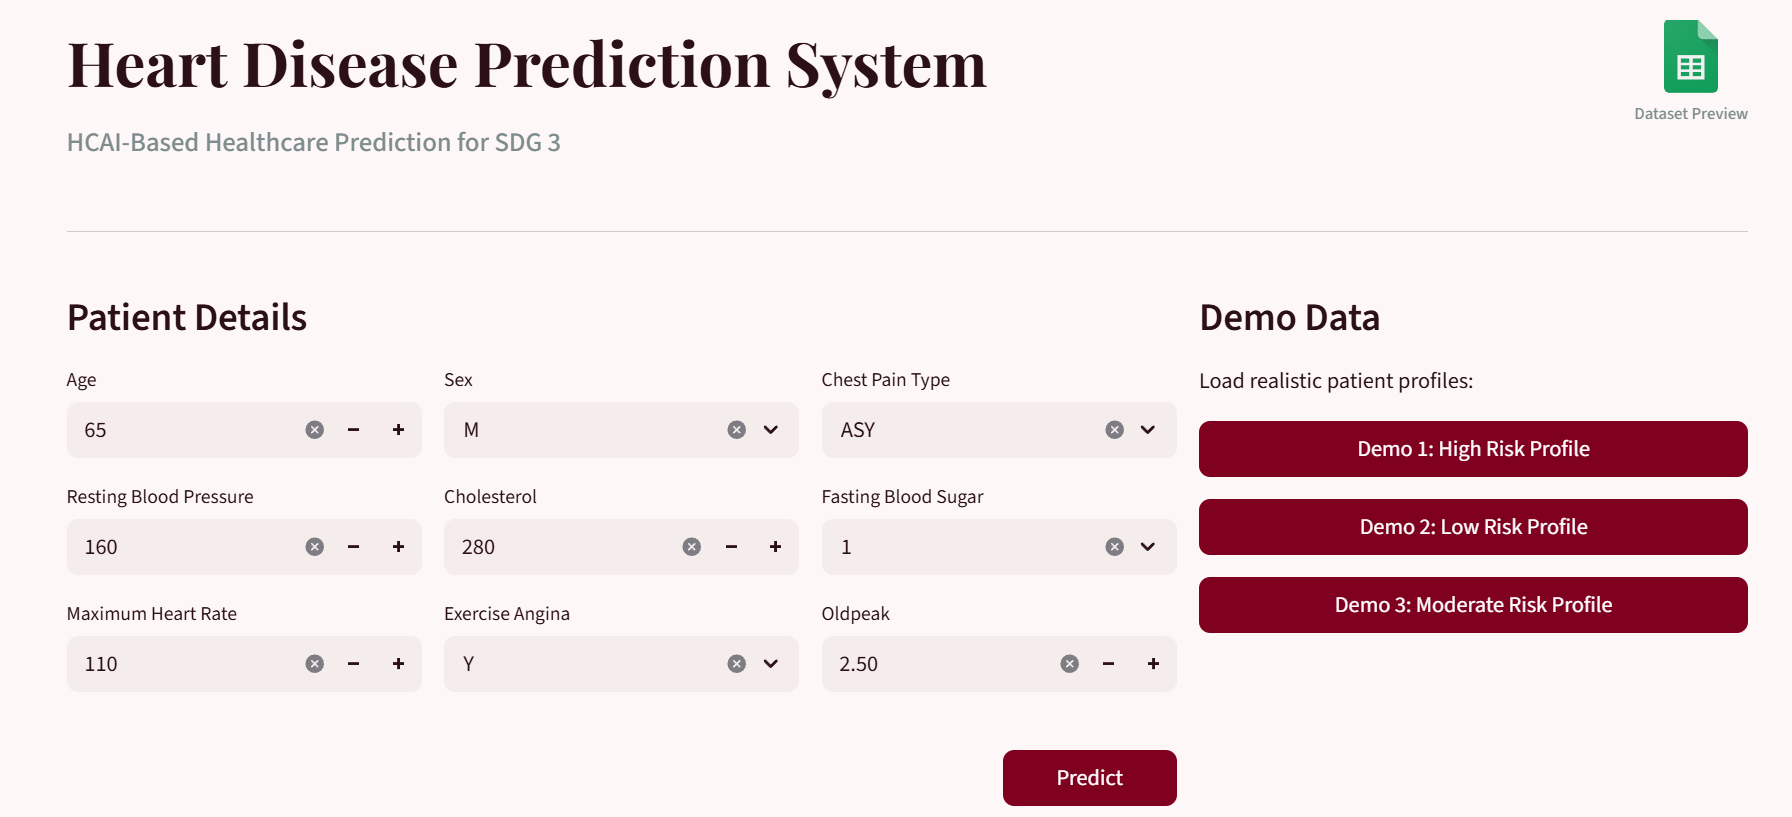
\includegraphics[width=0.95\textwidth]{frontend_interface.png}
\caption{Frontend Interface of the Heart Disease Prediction System}
\end{figure}

\vspace{0.5cm}

\subsection*{High Risk Prediction Output}

When the entered patient metrics indicate a high probability of heart disease, the system displays a high-risk warning message along with the calculated probability score and healthcare recommendation. The interface uses color-coded visual indicators to improve readability and risk awareness.

\begin{figure}[h]
\centering
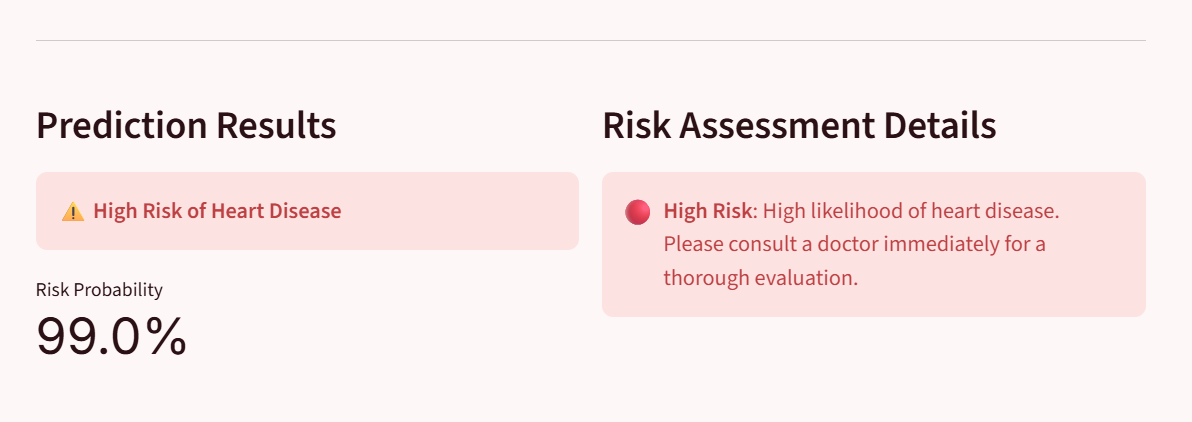
\includegraphics[width=0.85\textwidth]{high_risk_output.png}
\caption{High Risk Heart Disease Prediction Output}
\end{figure}

\vspace{0.5cm}

\subsection*{Low Risk Prediction Output}

When the patient metrics indicate a low probability of heart disease, the system displays a low-risk prediction with positive healthcare guidance and risk probability information.

\begin{figure}[h]
\centering
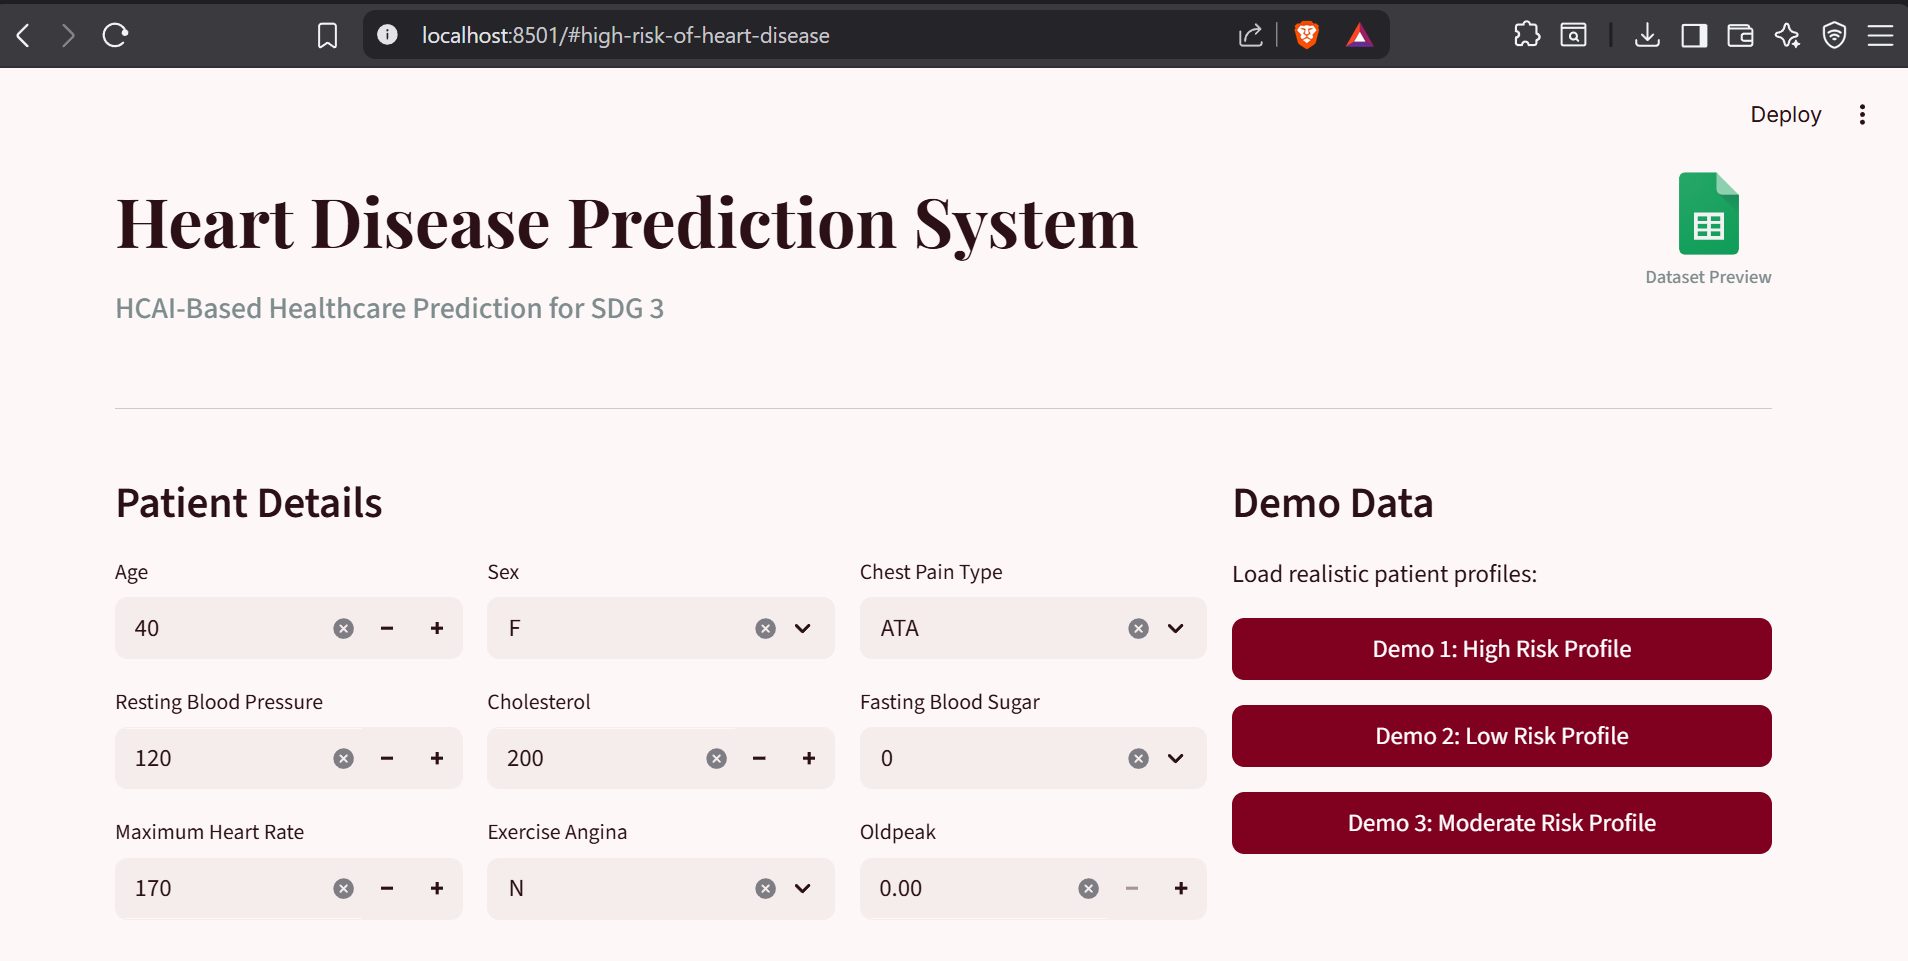
\includegraphics[width=0.95\textwidth]{low_risk_interface.png}
\caption{Low Risk Patient Input Example}
\end{figure}

\begin{figure}[h]
\centering
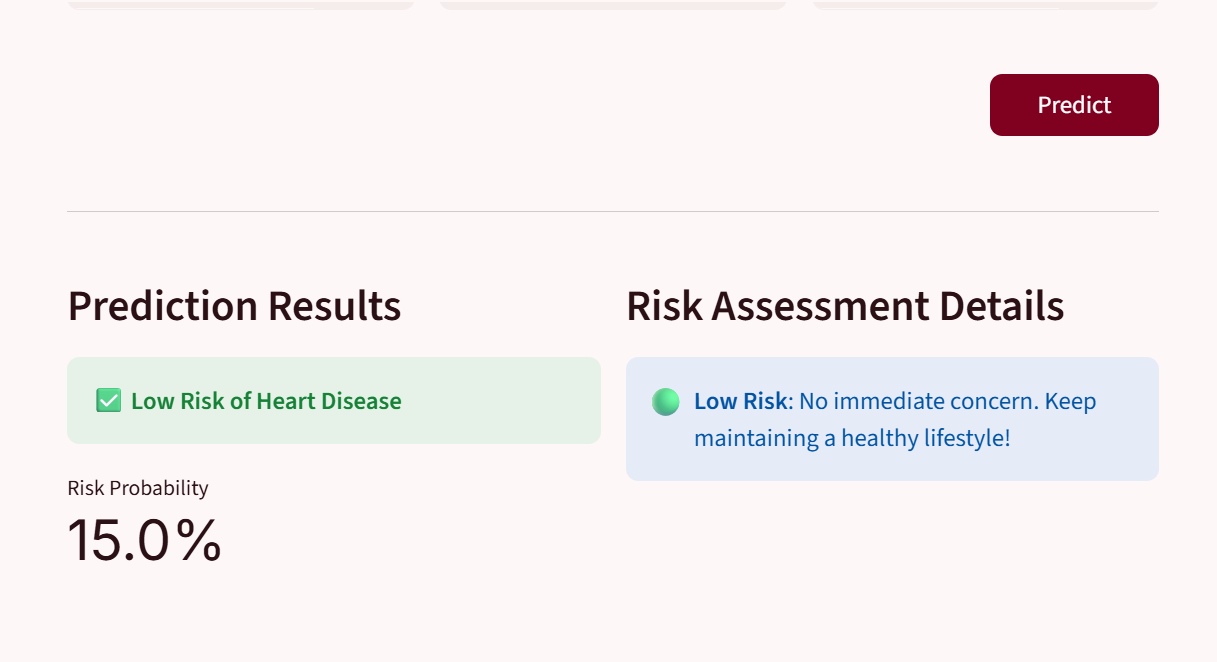
\includegraphics[width=0.85\textwidth]{low_risk_output.png}
\caption{Low Risk Heart Disease Prediction Output}
\end{figure}

\vspace{0.5cm}

The frontend emphasizes Human-Centered AI principles by providing:
\begin{itemize}
    \item User-friendly interaction
    \item Clear healthcare guidance
    \item Visual risk indicators
    \item Human-controlled prediction execution
    \item Explainable prediction outputs
\end{itemize}
\subsection*{Key Features}

\begin{itemize}
    \item Responsive web interface
    \item Real-time prediction
    \item User-friendly healthcare dashboard
    \item Risk probability visualization
    \item Demo profiles for testing
\end{itemize}

\section*{Detailed System Workflow}

\subsection*{1. Dataset Preparation}

\begin{itemize}
    \item Heart Disease dataset was collected and preprocessed.
    \item Categorical data was encoded using LabelEncoder.
    \item Numerical features were normalized where required.
\end{itemize}

\subsection*{2. Data Visualization}

The dataset was analyzed using:
\begin{itemize}
    \item Histograms
    \item Boxplots
    \item Correlation heatmaps
    \item Pair plots
\end{itemize}

\subsection*{3. Model Training}

\begin{itemize}
    \item The dataset was divided into training and testing sets.
    \item Multiple algorithms were trained and evaluated.
    \item Performance metrics were compared.
\end{itemize}

\subsection*{4. Frontend Prediction}

\begin{itemize}
    \item Users enter patient details.
    \item Input data is processed by the Random Forest model.
    \item Prediction and probability score are displayed.
\end{itemize}

\section*{Design Metaphors}

\subsection*{Clinical Assistant}

The application behaves like a lightweight healthcare assistant that helps users understand possible heart disease risks.

\subsection*{Risk Radar}

The prediction interface acts like a risk radar that visually highlights possible health risks.

\subsection*{Healthcare Dashboard}

The system interface resembles a healthcare dashboard with organized patient metrics and risk indicators.

\subsection*{Decision Support System}

The application supports human healthcare decisions without replacing medical professionals.

\section*{Ethics and Responsible AI}

\subsection*{Transparency}

\begin{itemize}
    \item The system clearly states that predictions are advisory.
    \item Risk probability is displayed openly.
\end{itemize}

\subsection*{Human Oversight}

\begin{itemize}
    \item Humans remain responsible for healthcare decisions.
    \item The AI system does not replace doctors.
\end{itemize}

\subsection*{Privacy}

\begin{itemize}
    \item No persistent patient data is stored.
    \item The application avoids collecting personally identifiable information.
\end{itemize}

\subsection*{Fairness and Bias Awareness}

\begin{itemize}
    \item Predictions depend on the quality of training data.
    \item Model bias and dataset limitations are acknowledged.
\end{itemize}

\section*{Accessibility Features}

\begin{itemize}
    \item Simple user interface for non-technical users.
    \item Clearly labeled input fields.
    \item Color-coded prediction indicators.
    \item Interactive and responsive design.
\end{itemize}

\section*{HCAI Best Practices Embedded}

\begin{itemize}
    \item Human control over prediction execution.
    \item Explainable risk outputs.
    \item Advisory rather than autonomous AI behavior.
    \item Ethical AI boundaries and disclaimers.
    \item Interactive user feedback.
\end{itemize}

\section*{Recommendations for Future Improvements}

\begin{itemize}
    \item Add explainable AI visualizations.
    \item Improve model interpretability.
    \item Add healthcare chatbot support.
    \item Expand dataset diversity.
    \item Include multilingual accessibility features.
\end{itemize}

\section*{Conclusion}

This Heart Disease Prediction System demonstrates how Human-Centered AI can support healthcare awareness while maintaining human oversight and ethical AI principles. The project combines machine learning, healthcare analytics, and accessible frontend design to create an educational and socially beneficial healthcare support system aligned with Sustainable Development Goals.

\end{document}